\documentclass[11pt,a4paper]{article}
% Status (2026-11-05): HISTORY: status note of 2026-11-02 (scripted carry plan; retired 11-03, see docs/status/2026-11-03_handoff_notes.md). Current claims: docs/paper/claims_2026-11-02.md.
\usepackage[margin=2.1cm]{geometry}
\usepackage[T1]{fontenc}
\usepackage{lmodern}
\usepackage{microtype}
\usepackage{booktabs}
\usepackage{tabularx}
\usepackage{graphicx}
\usepackage{amsmath,amssymb}
\usepackage[table]{xcolor}
\usepackage{enumitem}
\usepackage{hyperref}
\hypersetup{colorlinks=true,linkcolor=black,urlcolor=blue!50!black}
\setlist{itemsep=1pt,topsep=3pt}
\newcolumntype{Y}{>{\raggedright\arraybackslash}X}
\newcommand{\lab}[1]{\textsc{#1}}
\definecolor{bad}{HTML}{FBE7E4}
\definecolor{good}{HTML}{E3EFE8}
\title{\textbf{Certified segments for hidden-contents carrying}\\[2pt]
\large What we propose, how it treats the coffee-tray task, and how AgentChord does on it}
\author{Bimanual NERO project (simulation only) \quad--- status note, 2 Nov 2026}
\date{}
\begin{document}
\maketitle
\vspace{-1.5em}

\section*{Summary}
\begin{itemize}
\item \textbf{The problem.} A robot carries a tray of mugs, or a box, whose contents it cannot see. The contents mass and
centre of mass (COM) change what is safe: one arm or two, how fast, and whether to do it at all. AgentChord (arXiv 2605.11951),
our main baseline, plans the coffee-tray task with an LLM and watches it with pose checks only. It never reasons about mass,
force or torque.
\item \textbf{What we propose.} Split the task into segments (lift, carry, place, release). Before a segment runs, the robot
holds a \emph{stored backup} ("let go in place"). It runs the segment only if a certificate shows that, for every contents
value in its belief set, neither the segment nor the backup (from any point of the segment) enters the unsafe set $U$, and
both end at rest in $R$. The static rows are exact corner checks (proof under a stated model). The dynamic rows are
simulated (sampled, with $n$).
\item \textbf{AgentChord on its own coffee tray (our re-run, GPT-5.6, in its own simulator).} With a detailed prompt the plan
works (12/12). With the paper's one-line prompt it fails (0/12 strict). Under disturbances: capsule slide-out 0/18 (all
silent), doubled tray mass 0/18, five-times mass 0/18, bump 2/18. Its "holding" monitor counts an \emph{open, empty} gripper as
holding.
\item \textbf{Our certificate on the tray and box (no runtime yet).} The contents now change the action: 2- and 4-mug trays are
admitted with two arms for every fill; the 6-mug tray only up to 50~g per mug; the box only up to 2.0~kg. Above that we refuse.
With the controller fix below, every admitted cell held in simulation: 0/20 nominal runs unsafe and 0 failed backups out of
260--320 backup branches per cell; all 20 worlds per cell end at rest (sampled; per-segment Clopper--Pearson bound
$\varepsilon\le0.139$ at $n=20$).
\item \textbf{Two corrections we owe.} (1) The first sampled run failed many box worlds by tilt. The cause was our controller
(wrist stiction that FL-MPC does not model), not the contents. A friction-compensation wrapper cuts box tilt from 18.7$^\circ$
to 1.85$^\circ$. (2) With that fix, an AgentChord-style executor runs the box cells we refuse at 2.0--3.5~kg and both refused
6-mug cells with 0/20 unsafe each \emph{in simulation}. Those refusals rest on an \lab{assumed} claw-twist cap (1.3~Nm) and the
datasheet payload, neither of which the rigid-weld simulation can violate. The simulation cannot tell whether they are right; a
hardware or contact-model test must. From 3.5~kg up the simulation agrees with us: the executor fails 4/20, 9/20 and 17/20.
\end{itemize}

%=====================================================================
\section{The coffee-tray task and how an AgentChord plan looks}
AgentChord's coffee-tray task: the left arm puts a coffee capsule into a tray, then both arms lift the tray, carry it 10~cm
forward and set it down. The paper reports 60\% success on its real robot. AgentChord builds a plan in three layers:
\begin{enumerate}
\item a \textbf{task graph} of states and actions, written by the LLM (GPT-5 in the paper; GPT-5.6-terra/sol in our re-run);
\item a \textbf{monitor} attached to some steps;
\item \textbf{recovery branches} compiled before the run. At run time a fired monitor jumps to one of them; nothing new is planned.
\end{enumerate}
Figure~\ref{fig:graph} shows one real plan (GPT-5.6-terra, detailed prompt; 6/6 successes without disturbance).

\begin{figure}[p]
\centering
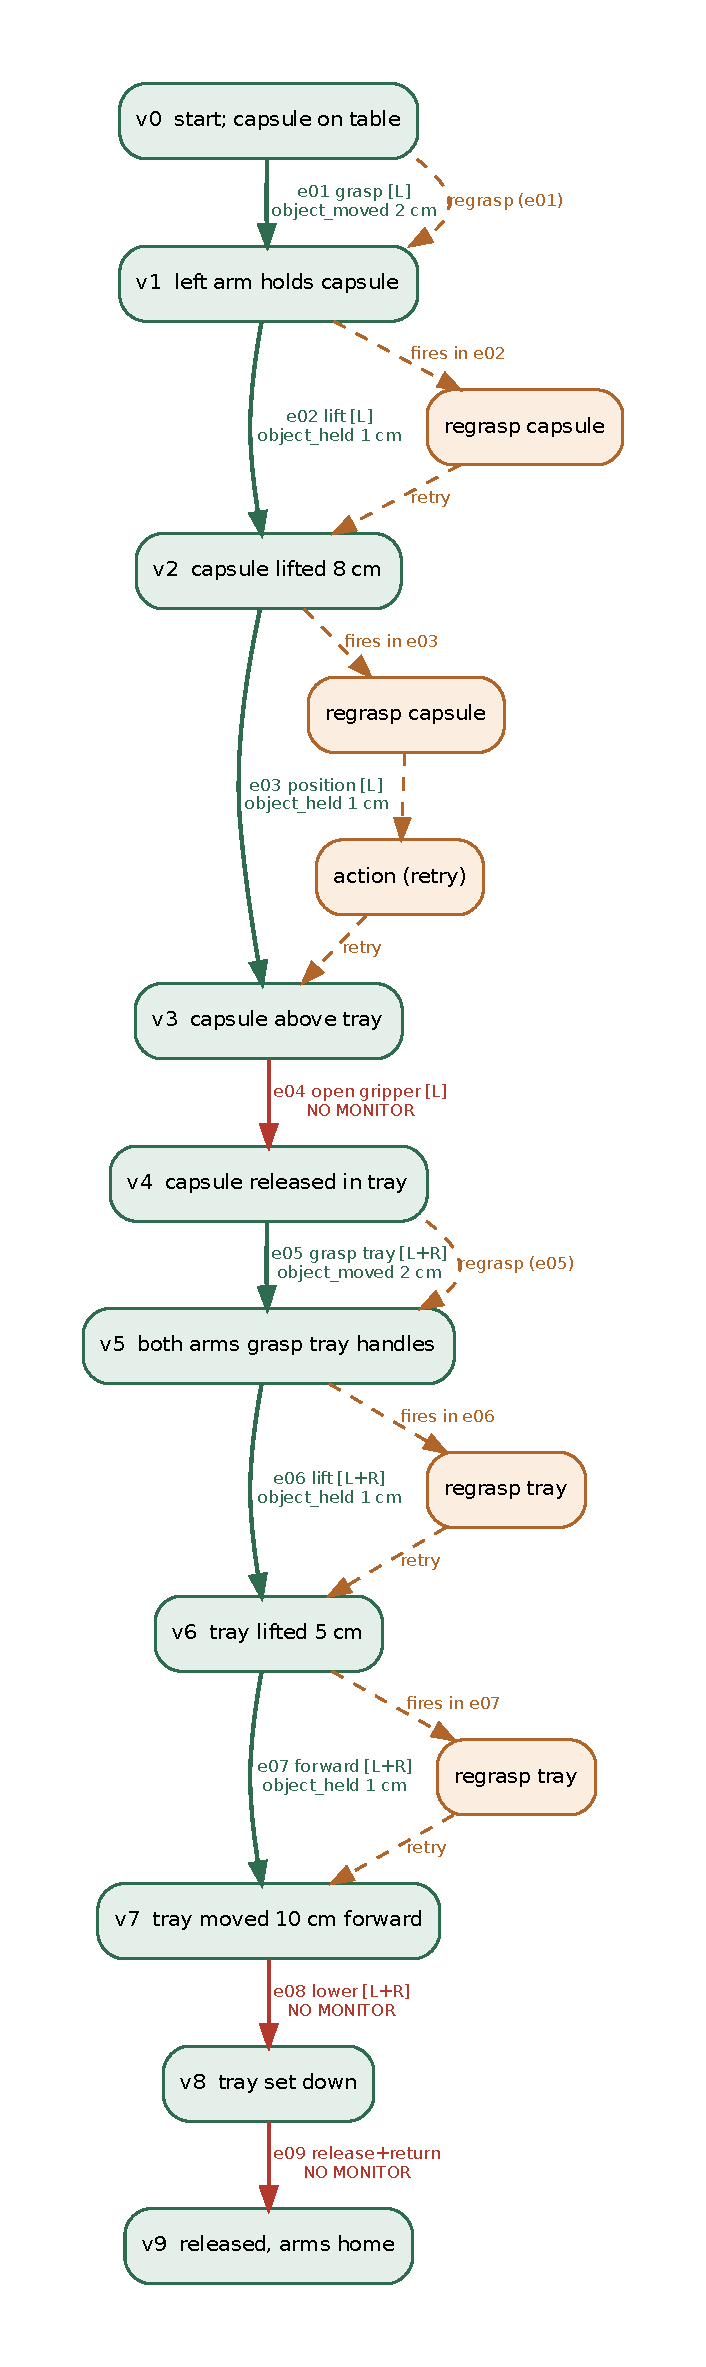
\includegraphics[height=0.80\textheight]{agentchord_plan.pdf}
\caption{One AgentChord plan for the coffee tray. Green: main path; red edges: steps with no monitor; orange dashed: recovery
branches written before the run. Redrawn from the plan file (some recovery self-loops omitted).}
\label{fig:graph}
\end{figure}

\begin{table}[h]
\centering\footnotesize
\begin{tabularx}{\linewidth}{@{}lYYll@{}}
\toprule
Step & Left arm & Right arm & Monitor (object, threshold) & Recoveries\\
\midrule
e01 grasp capsule & grasp(capsule, pre 0.05) & -- & object\_moved(capsule, 2 cm) & regrasp\\
e02 lift capsule & offset dz $=0.08$ & -- & object\_held(capsule, 1 cm) & regrasp, retry\\
e03 position in tray & move rel.\ tray (0, 0.06, 0.10) & -- & object\_held(capsule, 1 cm) & regrasp, action, retry\\
\rowcolor{bad} e04 release capsule & open\_gripper & -- & none & none\\
e05 grasp tray & grasp(tray) & grasp(tray) & object\_moved(tray, 2 cm) & regrasp\\
e06 lift tray & dz $=0.05$ & dz $=0.05$ & object\_held(tray, 1 cm) & regrasp, retry\\
e07 move forward & dx $=0.10$ & dx $=0.10$ & object\_held(tray, 1 cm) & regrasp, retry\\
\rowcolor{bad} e08 lower tray & dz $=-0.05$ & dz $=-0.05$ & none & none\\
\rowcolor{bad} e09 release+return & home & home & none & none\\
\bottomrule
\end{tabularx}
\caption{The same plan step by step. \texttt{object\_moved} fires when the object pose jumps more than 2~cm between checks.
\texttt{object\_held} fires when the gripper opening drops below 1~cm, so an open empty gripper still counts as holding.}
\end{table}

\paragraph{What the plan cannot see.}
\begin{itemize}
\item Releasing the capsule, lowering the tray and the final release have no monitor (red rows).
\item While the tray is carried only the grippers are watched. The capsule is never checked; if it slides out, the run continues.
\item Monitors are geometric only. Mass, force and joint torque never enter the plan, so a heavier tray is invisible until
something drops.
\item Recoveries are fixed regrasp or retry steps. None checks that the arm can reach the new pose, and the snap-to-reachable
option in the released code crashes (an \texttt{AttributeError}; dead code).
\end{itemize}

\begin{table}[h]
\centering\footnotesize
\begin{tabular}{@{}lrrrrr@{}}
\toprule
Plan & Main steps & Monitored & Unmonitored & Recovery steps & Recovery states\\
\midrule
full\_terra\_s11 & 9 & 7 & 2 & 23 & 8\\
full\_terra\_s12 & 9 & 6 & 3 & 16 & 5\\
full\_terra\_s13 & 9 & 4 & 5 & 8 & 2\\
full\_sol\_s11 & 9 & 7 & 2 & 23 & 8\\
full\_sol\_s12 & 9 & 7 & 2 & 23 & 8\\
full\_sol\_s13 & 9 & 6 & 3 & 18 & 6\\
min\_terra\_s11 & 7 & 4 & 3 & 8 & 2\\
min\_terra\_s12 & 7 & 4 & 3 & 8 & 2\\
min\_terra\_s13 & 9 & 5 & 4 & 11 & 3\\
min\_sol\_s11 & 10 & 5 & 5 & 21 & 7\\
min\_sol\_s12 & 11 & 7 & 4 & 26 & 9\\
min\_sol\_s13 & 7 & 4 & 3 & 11 & 3\\
\bottomrule
\end{tabular}
\caption{All 12 coffee-tray plans. Every plan uses only the two monitor types above. The same prompt and model can give 8 or 23
recovery steps. ``full'' = detailed prompt, ``min'' = the paper's one-line instruction; sol plans had object names resolved.}
\end{table}

%=====================================================================
\section{How badly AgentChord does on the coffee tray (its own simulator)}
Setup (28 Oct): AgentChord's released code and simulator, GPT-only through Codex (\texttt{gpt-5.6-terra}, \texttt{gpt-5.6-sol};
Codex adds its own system prompt and its temperature cannot be set). The paper used GPT-5. Our numbers are therefore for
AgentChord's \emph{mechanism} with a newer proposer, not a reproduction of its paper numbers.

\paragraph{Prompting.} Detailed prompt (numeric offsets written by a human, fair layout): 12/12 strict. The paper's one-line
real-robot prompt: 2/12 loose, 0/12 strict. The failures were graph-validator rejections and IK crashes inside moves the
planner chose (e.g.\ forward 0.2~m with no lift).

\begin{table}[h]
\centering\small
\begin{tabular}{@{}llp{8.3cm}@{}}
\toprule
Disturbance (18 episodes each) & Success & What happened\\
\midrule
drop, 10\% & 18/18 & only 2 drops were actually applied, so this says little\\
\rowcolor{bad} capsule slides out of the tray & 0/18 & 18/18 silent: no monitor watches the capsule while the tray moves\\
nudge 4 cm & 18/18 & pose monitor + regrasp handle it\\
\rowcolor{bad} bump & 2/18 & \\
\rowcolor{bad} tray mass $\times 2$ & 0/18 & monitor fired in 18; 6 runs crashed\\
\rowcolor{bad} tray mass $\times 5$ & 0/18 & monitor fired; 10 runs crashed\\
\bottomrule
\end{tabular}
\caption{Disturbance sweep: 108 episodes with full-prompt plans.}
\end{table}

\paragraph{Why it fails.}
\begin{enumerate}
\item \textbf{Hold check is width only.} \texttt{hold\_lost} = gripper opening below a threshold. An open, empty gripper counts as
holding; in some runs it ``carried'' the tray with open grippers, silently.
\item \textbf{No physics in admission.} Nothing checks mass, payload, torque or support before acting; a heavier tray is
discovered by failing.
\item \textbf{Recoveries are not checked.} Regrasp targets are often IK-infeasible; the reachability fallback is dead code.
\item \textbf{Unwatched steps.} Release, lower and final release carry no monitor in most plans.
\item \textbf{Brittle release.} The shipped example plans are stale (the \texttt{hold\_lost} threshold changed after they were written).
\end{enumerate}

%=====================================================================
\section{The approach we propose}
\subsection{Problem statement}
\begin{itemize}
\item \textbf{World.} Robot, tray/box geometry and the support surfaces are known. The \emph{contents} are hidden: mass per mug
(tray) or contents mass (box) lies in an interval, and the COM may be anywhere inside the container. The grasp is a rigid weld
once closed (\lab{assumed}, user decision 1 Nov: wrist cameras and low-level control own grasping).
\item \textbf{Belief.} A belief cell $\Theta$ = contents-mass interval $\times$ the full COM set. In the inertial parameters
$\pi=(m, m c)$ this set is convex, so a check that is linear in $\pi$ holds on the whole cell iff it holds at its corners.
\item \textbf{Task.} A sequence of segments: lift, carry, place, release (tray: lift 5~cm, carry 10~cm, place; box: lift 18~cm,
carry 20~cm over a shelf, place).
\item \textbf{Unsafe set $U$.} Any joint torque at the 16~Nm limit; object tilt $>10^\circ$ (\lab{assumed}) or a drop; a mug
tipped $>20^\circ$ or off the tray; spill proxy $(D/2)\tan\phi >$ freeboard; arm collision.
\item \textbf{Rest set $R$.} Object resting on a support, speed $<5$~mm/s, tilt $<3^\circ$, mugs upright within $5^\circ$, not in $U$.
\end{itemize}

\subsection{Admission rule (per segment)}
Before segment $s$ starts, the robot holds a stored backup $b_s$. The segment is admitted iff
\begin{align*}
\forall \theta\in\Theta:\quad & \underbrace{\xi_s(\theta)\cap U=\emptyset\ \text{ and }\ \xi_s(\theta)\ \text{ends in } R}_{\text{nominal segment}}\\
\text{and}\quad \forall x\in\xi_s(\theta):\quad & \underbrace{\xi_{b_s}(x,\theta)\cap U=\emptyset\ \text{ and }\ \xi_{b_s}(x,\theta)\ \text{ends in } R}_{\text{stored backup started from any point of the segment}}
\end{align*}
where $\xi_s(\theta)$ is the segment's trajectory in world $\theta$ and $\xi_{b_s}(x,\theta)$ the backup's trajectory from state $x$.
The backup is chosen \emph{before} the segment and does not depend on $\theta$. If no admitted action exists, the robot refuses
and stays where it is, which is already at rest in $R$.

\paragraph{Stored backups (``let go in place'').} Stop (decelerate the commanded reference) $\to$ retrace to the segment-start
poses stored at admission $\to$ hold $\to$ open (weld off) $\to$ retreat 5~cm $\to$ hold. Every target was reached before, so
there is nothing to choose at trigger time and no reachability gamble. Release has no backup.

\subsection{How the certificate is checked}
\begin{center}\small
\begin{tabularx}{\linewidth}{@{}lYl@{}}
\toprule
Row & What it checks & Guarantee type\\
\midrule
torque / payload / twist & $\tau_i = G_i + M_iJ_i^{+}[a;0] + J_i^\top w_i$ at 7 path samples, over the cell corners $\times$ the
acceleration box; joint $|\tau|\le 16$~Nm, payload $\le 2.5$~kg per arm, claw twist $\le 1.3$~Nm, admitted at $u\le 0.9$
& proof under MODEL\\
support at destination & COM of the object over the destination support polygon, all corners & proof under MODEL\\
open contents & quasi-static liquid surface vs freeboard at the planned acceleration & proof under MODEL (no slosh)\\
dynamics + backups & MuJoCo, $n=20$ worlds per admitted cell, backups branched every 0.25~s & sampled ($n$, Clopper--Pearson)\\
\bottomrule
\end{tabularx}
\end{center}
``Proof under MODEL'' means: for all $\theta$ in the cell, under the stated quasi-static rigid-weld model with the NERO MJCF arms.
It is not a proof about the real robot. A simulated failure \emph{refutes} an admission.

\subsection{Action rule}
For each cell the robot picks the first admitted option in the order: one arm $\to$ two arms with a lever split $\to$ refuse.
The \textbf{lever split} gives each claw the force and twist that a rigid lever between the two claws needs to carry the load
(linear in $\pi$). The older 50/50-at-COM split commanded about 1.2~Nm of internal twist per claw for nothing and is superseded.

%=====================================================================
\section{How this helps the coffee case}
Our tray task is the carrying half of the coffee tray, with the part AgentChord ignores made explicit: the mugs (or the capsule)
have unknown mass and position. Each AgentChord failure maps to a mechanism:

\begin{center}\small
\begin{tabularx}{\linewidth}{@{}YY>{\raggedright\arraybackslash}p{3.3cm}@{}}
\toprule
AgentChord failure on the coffee tray & What our approach does instead & Status\\
\midrule
Heavier tray ($\times2$, $\times5$): 0/18, crashes & Contents are a belief cell; the torque/payload/twist row is checked for every
corner \emph{before} lifting; the action becomes two arms or refuse & built (static rows, proof under MODEL)\\
Recoveries IK-infeasible; snap fallback dead & Backup targets are poses already reached at segment start, stored and simulated
at admission & built (sampled, $n=20$/cell)\\
Release / lower / final release unmonitored & Every segment has $U$ and $R$ checks; lift, carry and place each have a backup &
built; release has no backup\\
Capsule slide-out, 0/18 silent & Mugs off the tray or tipped are in $U$; the sampled rows simulate them for every admitted cell;
a mug not upright fails $R$ & built offline; runtime detection needs ZED tracking of the mugs (not built)\\
``Open empty gripper = holding'' & The hold is read from the claw wrench (weld force balances the weight within 5\% in the test),
not the gripper width & built in sim; grasp itself is \lab{assumed} rigid\\
Same prompt gives 8 or 23 recovery steps & Backups are a fixed library per segment type; the proposer (LLM) may propose, only the
certificate admits & library built; proposer not yet in this loop\\
\bottomrule
\end{tabularx}
\end{center}

\noindent\textbf{What it does not yet do for the coffee case:} no runtime trigger loop for the tray (the certificate is used as
an offline admission check; the trigger runtime exists only in the pan plan), no belief narrowing from joint torques, no capsule
placement step, and the grasp is welded, so grasp slip is out of scope by assumption.

%=====================================================================
\section{Results so far (simulation, 1--2 Nov)}
\subsection{Action thresholds (worst COM, proof under MODEL)}
\begin{center}\small
\begin{tabular}{@{}ll@{}}
\toprule
Object & Decision by contents mass\\
\midrule
pan & one arm $\le 0.22$~kg, else refuse\\
pot (two handles) & one arm $\le 0.20$~kg; two arms (lever) $\le 2.63$~kg; else refuse\\
tray, 2 or 4 mugs & always two arms (one arm refused by the twist cap)\\
tray, 6 mugs & two arms $\le 2.3$~kg in mugs, else refuse\\
box onto shelf & two arms $\le 2.38$~kg, else refuse\\
\bottomrule
\end{tabular}
\end{center}

\subsection{Per-cell certificate}
\begin{center}\small
\footnotesize\begin{tabular}{@{}lllp{3.0cm}cccc@{}}
\toprule
 & & & & \multicolumn{2}{c}{No friction comp.} & \multicolumn{2}{c}{With friction comp.}\\ \cmidrule(l){5-6}\cmidrule(l){7-8}
Cell (contents) & Static & $u_{\rm nom}$ & Binding row & nom.\ $U$ & bad backup & nom.\ $U$ & bad backup\\
\midrule
tray2, 0--50 g/mug & two & 0.65 & -- & 0/20 & 0/20 & \textbf{0/20} & \textbf{0/20}\\
tray2, 50--125 g & two & 0.67 & -- & 0/20 & 1/20 & \textbf{0/20} & \textbf{0/20}\\
tray2, 125--250 g & two & 0.70 & -- & 2/20 & 2/20 & \textbf{0/20} & \textbf{0/20}\\
tray4, 0--50 g & two & 0.74 & -- & 0/20 & 0/20 & \textbf{0/20} & \textbf{0/20}\\
tray4, 50--125 g & two & 0.78 & -- & 1/20 & 1/20 & \textbf{0/20} & \textbf{0/20}\\
tray4, 125--250 g & two & 0.85 & -- & 2/20 & 3/20 & \textbf{0/20} & \textbf{0/20}\\
tray6, 0--50 g & two & 0.84 & -- & 1/20 & 1/20 & \textbf{0/20} & \textbf{0/20}\\
\rowcolor{bad} tray6, 50--125 g & refuse & 0.98 & payload (left arm 23.9 of 24.5 N) & -- & -- & -- & --\\
\rowcolor{bad} tray6, 125--250 g & refuse & 1.24 & payload & -- & -- & -- & --\\
box 0.5--1.0 kg & two & 0.71 & -- & 18/20 & 20/20 & \textbf{0/20} & \textbf{0/20}\\
box 1.0--1.5 kg & two & 0.79 & -- & 16/20 & 20/20 & \textbf{0/20} & \textbf{0/20}\\
box 1.5--2.0 kg & two & 0.88 & -- & 11/20 & 20/20 & \textbf{0/20} & \textbf{0/20}\\
\rowcolor{bad} box 2.0--5.0 kg (6 cells) & refuse & 1.01--2.02 & claw twist 1.32--2.63 Nm (cap 1.3, \lab{assumed}) & -- & -- & -- & --\\
\bottomrule
\end{tabular}
\end{center}
``two'' = two arms with the lever split. Every sampled failure in that run was object tilt $>10^\circ$. Lighter boxes failed \emph{more} often, which pointed at the
controller, not the contents.

\subsection{Tilt: root cause and fix}
On a 0.59~kg box the commanded orientation is constant ($0.00^\circ$) but the box tilts $14^\circ$; wrist joints j5/j6 lag by
0.2--0.3~rad, the same with one weld or with the payload feed-forward off. FL-MPC has no joint-friction model, and the wrists
have tiny inertia (about 1~Nm/rad effective stiffness) against the MJCF friction loss of 0.3~Nm, so they stall. Fix: a wrapper
after FL-MPC (FL-MPC itself unchanged) adds $\tau = f\tanh(\dot q_{\rm cmd}/v_s) + k_i\!\int\! e + k_p e$, clipped to the torque
box; gains $f=0.3$ (= MJCF friction loss), $v_s=0.02$, $k_i=8$, $|{\int}|\le 0.6$, $k_p=5$ (\lab{assumed}).
\begin{center}\small
\begin{tabular}{@{}lcc@{}}
\toprule
Variant (same world, lift + carry) & Max tilt & End joint error\\
\midrule
none & 18.7$^\circ$ & 0.30 rad\\
friction feed-forward & 7.3$^\circ$ & 0.12 rad\\
+ integral & 3.7$^\circ$ & 0.036 rad\\
+ integral + P (used) & 1.85$^\circ$ & 0.023 rad\\
\bottomrule
\end{tabular}
\end{center}
With the fix, the certificate re-run (same cells, same worlds, $n=20$ per cell) has no unsafe nominal run and no failed backup
in any admitted cell (Section 5.2, right columns). Maximum object tilt over all runs: 1.5--3.3$^\circ$ on the trays and
3.5--5.7$^\circ$ on the box, against the $10^\circ$ limit; maximum joint torque 0.60--0.69 of 16~Nm.

\paragraph{Caveat: twist in the simulation.} The model row checks the twist we \emph{command} through the lever split. In the
simulation the welded closed chain adds internal twist, and the measured claw twist in admitted cells reaches 1.33--1.45~Nm on the
4- and 6-mug trays and up to 2.2~Nm on the box, above the 1.3~Nm cap. If the cap is real, those runs would slip on the robot.
So the twist cap is not yet enforced end to end: the controller needs an internal-force term, or the claw-wrench row must enter
$U$ (\texttt{strict\_claw}), before admitted cells can claim it.

\subsection{AgentChord-style executor on the cells we refuse}
This is \emph{not} AgentChord itself (its planner needs GPT and a GPU; not re-run here). It is its mechanism on our tasks: the
same plan, controller, speed and worlds as ours, no admission check, and its single-step pose monitor (object moved $>1$~cm
relative to the claw between steps). Under the weld it can fire only after the arms have already lost the box.
\begin{center}\small
\begin{tabular}{@{}l>{\raggedright\arraybackslash}p{3.3cm}>{\raggedright\arraybackslash}p{6.0cm}c@{}}
\toprule
Refused cell & Unsafe, no friction comp.\ & Unsafe, with friction comp. & Monitor fired (with fc)\\
\midrule
box 2.0--2.5 kg & 16/20 & 0/20 (max tilt 6.9$^\circ$, twist 2.6 Nm) & 0\\
box 2.5--3.0 kg & 15/20 & 0/20 (8.9$^\circ$, 3.0 Nm) & 0\\
box 3.0--3.5 kg & 16/20 & 0/20 (8.3$^\circ$, 3.3 Nm) & 0\\
box 3.5--4.0 kg & 18/20 & 4/20 (tilt; max 32$^\circ$) & 0\\
box 4.0--4.5 kg & 18/20 & 9/20 (6 tilt, 3 torque saturation; max 91$^\circ$) & 1\\
box 4.5--5.0 kg & 20/20 (9 by torque saturation) & 17/20 (10 torque saturation, 7 tilt; max 93$^\circ$) & 7\\
tray6, 50--125 g & 0/20 & 0/20 & 0\\
tray6, 125--250 g & 4/20 & 0/20 & 0\\
\bottomrule
\end{tabular}
\end{center}

\paragraph{How to read this.}
\begin{itemize}
\item Without the friction fix, most of the baseline's failures came from the same controller bug that hurt our admitted cells.
They are not evidence for our refusals.
\item With the fix, the box at 2.0--3.5~kg and the 6-mug tray run safely in simulation, \emph{without} our check. Our refusals
there come from two limits the simulation does not contain: the claw-twist cap (\lab{assumed} 1.3~Nm; the sim twist reaches
2.6--3.3~Nm, which a rigid weld always holds) and the datasheet payload (3~kg incl.\ the 0.5~kg gripper; the sim arm is limited only
by 16~Nm joint torque). So in these cells the refusal is conservative \emph{in sim} and right only if those limits are right on
the robot. That is a question for hardware or a slip-capable contact model, not for this simulation.
\item Joint torque, which the sim does model, starts to fail at 3.5--4.0~kg (4/20) and saturates at 4.5--5.0~kg (17/20 unsafe).
There our refusal and the simulation agree.
\item The baseline's monitor fired in 0 runs up to 3.5--4.0~kg, so those tips were silent. It fired in 1 and 7 runs at 4.0--5.0~kg,
only after the arms saturated and the weld stretched (1.6--1.7~cm per step), that is, after the box was already falling.
\end{itemize}

%=====================================================================
\section{Bounds and assumptions}
\begin{center}\small
\begin{tabularx}{\linewidth}{@{}>{\raggedright\arraybackslash}p{6.4cm}Yl@{}}
\toprule
Value & Bound on & Label\\
\midrule
16 Nm joint torque, 3 kg payload (2.5 kg net), 40 N claw & NERO datasheet (MIT $t_{ff}$ range) & MEASURED (spec)\\
rigid weld once the claw closes & grasp & \lab{assumed} (user, 1 Nov)\\
claw twist cap 1.3 Nm & claw, from the VIZ-COAST capacity fit extrapolated to 40 N & \lab{assumed} (approved 2 Nov)\\
admit at $u\le0.9$ & margin on the model rows & \lab{assumed} (approved 2 Nov)\\
$a_{\rm nom}=0.5$ m/s$^2$; mug 300 g / 250 ml / 1 cm freeboard & plan, objects & \lab{assumed} (approved 2 Nov)\\
tilt $10^\circ$ in $U$; backup decel 0.25 m/s$^2$; min admitted speed 0.05 & unsafe set, backup, action & \lab{assumed} (new, to confirm)\\
counter half-width 0.15 m, shelf 0.14 m & support geometry & \lab{assumed} (new, to confirm)\\
fill cells 0--50 / 50--125 / 125--250 g per mug & belief cells & \lab{assumed} (new, to confirm)\\
friction-compensation gains & controller wrapper & \lab{assumed} (new, to confirm)\\
quasi-static envelope, no slosh & model rows & MODEL\\
\bottomrule
\end{tabularx}
\end{center}
The friction-compensation torques (up to 0.9~Nm) are not in the static torque row; they fit inside the 0.9 margin. Comparisons
in Section 5 use the same worlds (seeds fixed per task, cell and index) for ours and the baseline.

\section{Next steps}
\begin{enumerate}
\item Close the twist gap: an internal-force term in the controller, or the claw-wrench row in $U$, then re-certify.
\item Decide how to test the twist cap and payload refusals: a slip-capable claw contact model (Drake was 40$\times$ lower creep
than MuJoCo in our spike) or a bench measurement.
\item Runtime loop for the tray: trigger monitors on encoders and claw wrench, belief narrowing from joint torques, then the
capsule placement step, so the full coffee-tray task runs end to end against AgentChord on the same worlds.
\end{enumerate}

\vfill
\footnotesize\sloppy\noindent Code: \texttt{world\_model/v2/nero/contents/} (envelope, thresholds, scenes, carry, carry\_cert,
baseline\_ungated, compare); results \texttt{world\_model/v2/nero/results/contents\_*\_2026-11-0\{1,2\}}; raw runs on westeros
\texttt{/data/local/ss5772/contents/}. AgentChord probe: \texttt{world\_model/v2/agentchord\_probe/}. All simulation; no hardware.
\end{document}
